\documentclass[12pt]{article}

\include{preamble}
\usepackage{float}

\newtoggle{professormode}
% \toggletrue{professormode} %STUDENTS: DELETE or COMMENT this line



\title{MATH 342W / 642 / RM 742 Spring \the\year ~HW \#3}

\author{Ye Htut Maung} %STUDENTS: write your name here

\iftoggle{professormode}{
\date{Due noon March 19 \\ \vspace{0.5cm} \small (this document last updated \currenttime~on \today)}
}

\renewcommand{\abstractname}{Instructions and Philosophy}

\begin{document}
\maketitle

\iftoggle{professormode}{
\begin{abstract}
The path to success in this class is to do many problems. Unlike other courses, exclusively doing reading(s) will not help. Coming to lecture is akin to watching workout videos; thinking about and solving problems on your own is the actual ``working out.''  Feel free to \qu{work out} with others; \textbf{I want you to work on this in groups.}

Reading is still \textit{required}. You should be googling and reading about all the concepts introduced in class online. This is your responsibility to supplement in-class with your own readings.

The problems below are color coded: \ingreen{green} problems are considered \textit{easy} and marked \qu{[easy]}; \inorange{yellow} problems are considered \textit{intermediate} and marked \qu{[harder]}, \inred{red} problems are considered \textit{difficult} and marked \qu{[difficult]} and \inpurple{purple} problems are extra credit. The \textit{easy} problems are intended to be ``giveaways'' if you went to class. Do as much as you can of the others; I expect you to at least attempt the \textit{difficult} problems. 

This homework is worth 100 points but the point distribution will not be determined until after the due date. See syllabus for the policy on late homework.

Up to 7 points are given as a bonus if the homework is typed using \LaTeX. Links to instaling \LaTeX~and program for compiling \LaTeX~is found on the syllabus. You are encouraged to use \url{overleaf.com}. If you are handing in homework this way, read the comments in the code; there are two lines to comment out and you should replace my name with yours and write your section. The easiest way to use overleaf is to copy the raw text from hwxx.tex and preamble.tex into two new overleaf tex files with the same name. If you are asked to make drawings, you can take a picture of your handwritten drawing and insert them as figures or leave space using the \qu{$\backslash$vspace} command and draw them in after printing or attach them stapled.

The document is available with spaces for you to write your answers. If not using \LaTeX, print this document and write in your answers. I do not accept homeworks which are \textit{not} on this printout. Keep this first page printed for your records.

\end{abstract}

\thispagestyle{empty}
\vspace{1cm}
NAME: \line(1,0){380}
\clearpage
}

\problem{These are questions about Silver's book, chapters 3-6.  For all parts in this question, answer using notation from class (i.e. $t ,f, g, h^*, \delta, \epsilon, e, t, z_1, \ldots, z_t, \mathbb{D}, \mathcal{H}, \mathcal{A}, \mathcal{X}, \mathcal{Y}, X, y, n, p, x_{\cdot 1}, \ldots, x_{\cdot p}$, $x_{1 \cdot}, \ldots, x_{n \cdot}$, etc.} % and also we now have $f_{pr}, h^*_{pr}, g_{pr}, p_{th}$, etc from probabilistic classification as well as different types of validation schemes)

\begin{enumerate}

\hardsubproblem{Chapter 4 is all about predicting weather. Broadly speaking, what is the problem with weather predictions? Make sure you use the framework and notation from class. This is not an easy question.}\spc{6}

One problem with weather prediction is that the weather system is dynamic, which means that one current behavior influences other behavior of the weather in the future. According to the chaos theorem, our errors are not changing in linear but exponential. If we use the same computer and one data is approximation of 3 decimal places and another data is 5 decimal place, the result can be completely different. Another problem is that there is a biases in a local news weather forecast. They prioritize customer sanctification over accuracy. For example, if there is 40\% chance of rain, they could raise up to 60\% of the rain. They usually predict rain more often than it actually occurs to appeal to consumers.

\easysubproblem{Why does the weatherman lie about the chance of rain? And where should you go if you want honest forecasts?}\spc{2}

The weatherman lies about the chance of rain because of economic incentives and consumer perception. For example, if there is 50\% chance of raining and the weatherman can lie about there is 60\% or 70\% of the rain. Many people will appreciate if the focus is going to rain and it will not rain in real time as it could help the morning commute or what to wear on that day. Otherwise people will blane to the weatherman. We should go to the National Wether Service if we want honest forecasts.

\hardsubproblem{Chapter 5 is all about predicting earthquakes. Broadly speaking, what is the problem with earthquake predictions? It is \textit{not} the same as the problem of predicting weather. Read page 162 a few times. Make sure you use the framework and notation from class.}\spc{5}

The problem with earthquake prediction is that we cannot look at the rock which is about fifteen kilometers underground to know what is happening there like weather forecasters do. That is the main problem to measure the stress. Seismologists use only statistical data to build a model but they cannot identify what are noises and what are signals. With the notation from the class, let $y$ be the earthquake occurs or not and $z$'s are the main cause which is the stress from the underground. However, we don't know $z$ and we use $x$ to predict $z$ which $x$ could be previous earthquakes data. Although we have $\mathbb{D}$ which is the historical data of earthquakes, we don't know if $x$ is the main cause to approximate $z$. That is the reason why I think predicting earthquake is impossible.

\easysubproblem{Silver has quite a whimsical explanation of overfitting on page 163 but it is really educational! What is the nonsense predictor in the model he describes?}\spc{2}

The nonsense predictor in the model he describes is the combination of red, black and blue locks. In the example, you can unlock the locks that he gave to you but it is too specific so that I can't open other locks.

\easysubproblem{John von Neumann was credited with saying that \qu{with four parameters I can fit an elephant and with five I can make him wiggle his trunk}. What did he mean by that and what is the message to you, the budding data scientist? }\spc{5}

It means that you are just in your imagination or in your delusion and you think that your model is very good like you can even make an elephant wiggle his trunk. You see a pattern to fit the elephant but actually you don't. The message to me is that you need to identify the noise carefully and not to overfit them and also even the errors are getting smaller, you model could be worse in generalization.

\hardsubproblem{Chapter 6 is all about predicting unemployment, an index of macroeconomic performance of a country. Broadly speaking, what is the problem with unemployment predictions? It is \textit{not} the same as the problem of predicting weather or earthquakes. Make sure you use the framework and notation from class.}\spc{6}

The problem with unemployment predictions is that economic systems are influenced by human behavior, policy decisions, and evolving market conditions. They are continuously changing and not stationary. Unlike weather or earthquakes, where physical laws provide consistency, economic relationships shift over time by unseen predictors. With notation, $t$, $f$, $h^*$ are always changeing.

\extracreditsubproblem{Many times in this chapter Silver says something on the order of \qu{you need to have theories about how things function in order to make good predictions.} Do you agree? Discuss.}\spc{13}


\end{enumerate}



\problem{These are questions related to the concept of orthogonal projection, QR decomposition and its relationship with least squares linear modeling.}

\begin{enumerate}

\easysubproblem{Let $\H$ be the orthogonal projection onto $\colsp{\X}$ where $\X$ is a $n \times (p+1)$ matrix with all columns linearly independent from each other. What is $\rank{\H}$?}\spc{0.5}

$\rank{\H}$ is $p + 1$ 


\easysubproblem{Simplify $\H\X$ by substituting for $\H$.}\spc{0.5}

\[
H X = X (X^T X)^{-1} X^T X
\]

\[
= X I \quad \text{(since \( A^{-1} A = I \))}
\]

\[
= X
\]

\intermediatesubproblem{What does your answer from the previous question mean conceptually?}\spc{2}

It means that since H is the projection matrix on column space of X, you are projecting into the same column space. In the class, we usually say we teleport the same room.

\hardsubproblem{Let $\X'$ be the matrix of $\X$ whose columns are in reverse order meaning that $\X = [ \onevec_n~\vdots~\x_{\cdot 1}~\vdots~ \ldots~\vdots~ \x_{\cdot p} ]$ and $\X' = [\x_{\cdot p}~\vdots~ \ldots~\vdots~\x_{\cdot 1}~\vdots~\onevec_n]$. Show that the projection matrix that projects onto $\colsp{X}$ is the same exact projection matrix that projects onto $\colsp{X'}$.}\spc{5}

Let
\[
H = X (X^T X)^{-1} X^T
\]

Let
\[
H' = X' (X'^T X')^{-1} X'^T
\]

\( H \) and \( H' \) apply to all the columns in \( X \) and \( X' \) as \( X \) and \( X' \) have the same information since they are just columns in reverse order.

Then, we extends $X$ to fill the $\mathbb{R}_n$ which we add $X_{\perp}$ 

\[
X_{\text{full}} = \begin{bmatrix} X & X_{\perp} \end{bmatrix}
\]

So,
\[
H X_{\text{full}} = \begin{bmatrix} X & 0_{n - (p+1)} \end{bmatrix}
\]

\[
H' X_{\text{full}} = \begin{bmatrix} X & 0_{n - (p+1)} \end{bmatrix}
\]

So, \( H \) and \( H' \) are the same because they get the same \( X \) in \( \mathbb{R}_n \).
Vice Visa, you can also extend  \( X' \) by adding $X'_{\perp}$ and use $H$ and $H'$ to project and you will get the same result of \( X' \).

\easysubproblem{Generalize the previous problem by proving that orthogonal projection matrices that project onto any specific subspace are \emph{unique}.}\spc{3}

Let \( U \) be a subspace of \( \mathbb{R}^n \) which has basis vectors \( u_1, u_2, u_3, \dots, u_q, \dots, u_n \).

\( P_1 \) is an orthogonal projection matrix on \( U \).  
\( P_2 \) is an orthogonal projection matrix on \( U \).

Let \( X \) be of dimension \( n \times (p+1) \), full rank, spanning the subspace \( U \).  
Let \( X_\perp \) be of dimension \( n \times (n - p -1) \), full rank, spanning the subspace \( U_\perp \).

\[
X_{\text{full}} = \begin{bmatrix} X & X_\perp \end{bmatrix}
\]
which is an \( n \times n \) matrix.

\[
P_1 X_{\text{full}} = \begin{bmatrix} X & 0_{n \times (n - p -1)} \end{bmatrix}
\]

\[
P_2 X_{\text{full}} = \begin{bmatrix} X & 0_{n \times (n - p -1)} \end{bmatrix}
\]

Thus, 
\[
P_1 X_{\text{full}} = P_2 X_{\text{full}}
\]
Since \( X \) is an \( n \times n \) full-rank matrix, we can multiply by its inverse:

\[
P_1 X_{\text{full}} X_{\text{full}}^{-1} = P_2 X_{\text{full}} X_{\text{full}}^{-1}
\]

\[
P_1 = P_2
\]

Thus, \( P_1 = P_2 \), proving that the orthogonal projection matrix onto any subspace is unique.



\easysubproblem{Prove that if a square matrix is both symmetric and idempotent then it must be an orthogonal projection matrix.}\spc{3}

\begin{figure}[H]
    \centering
    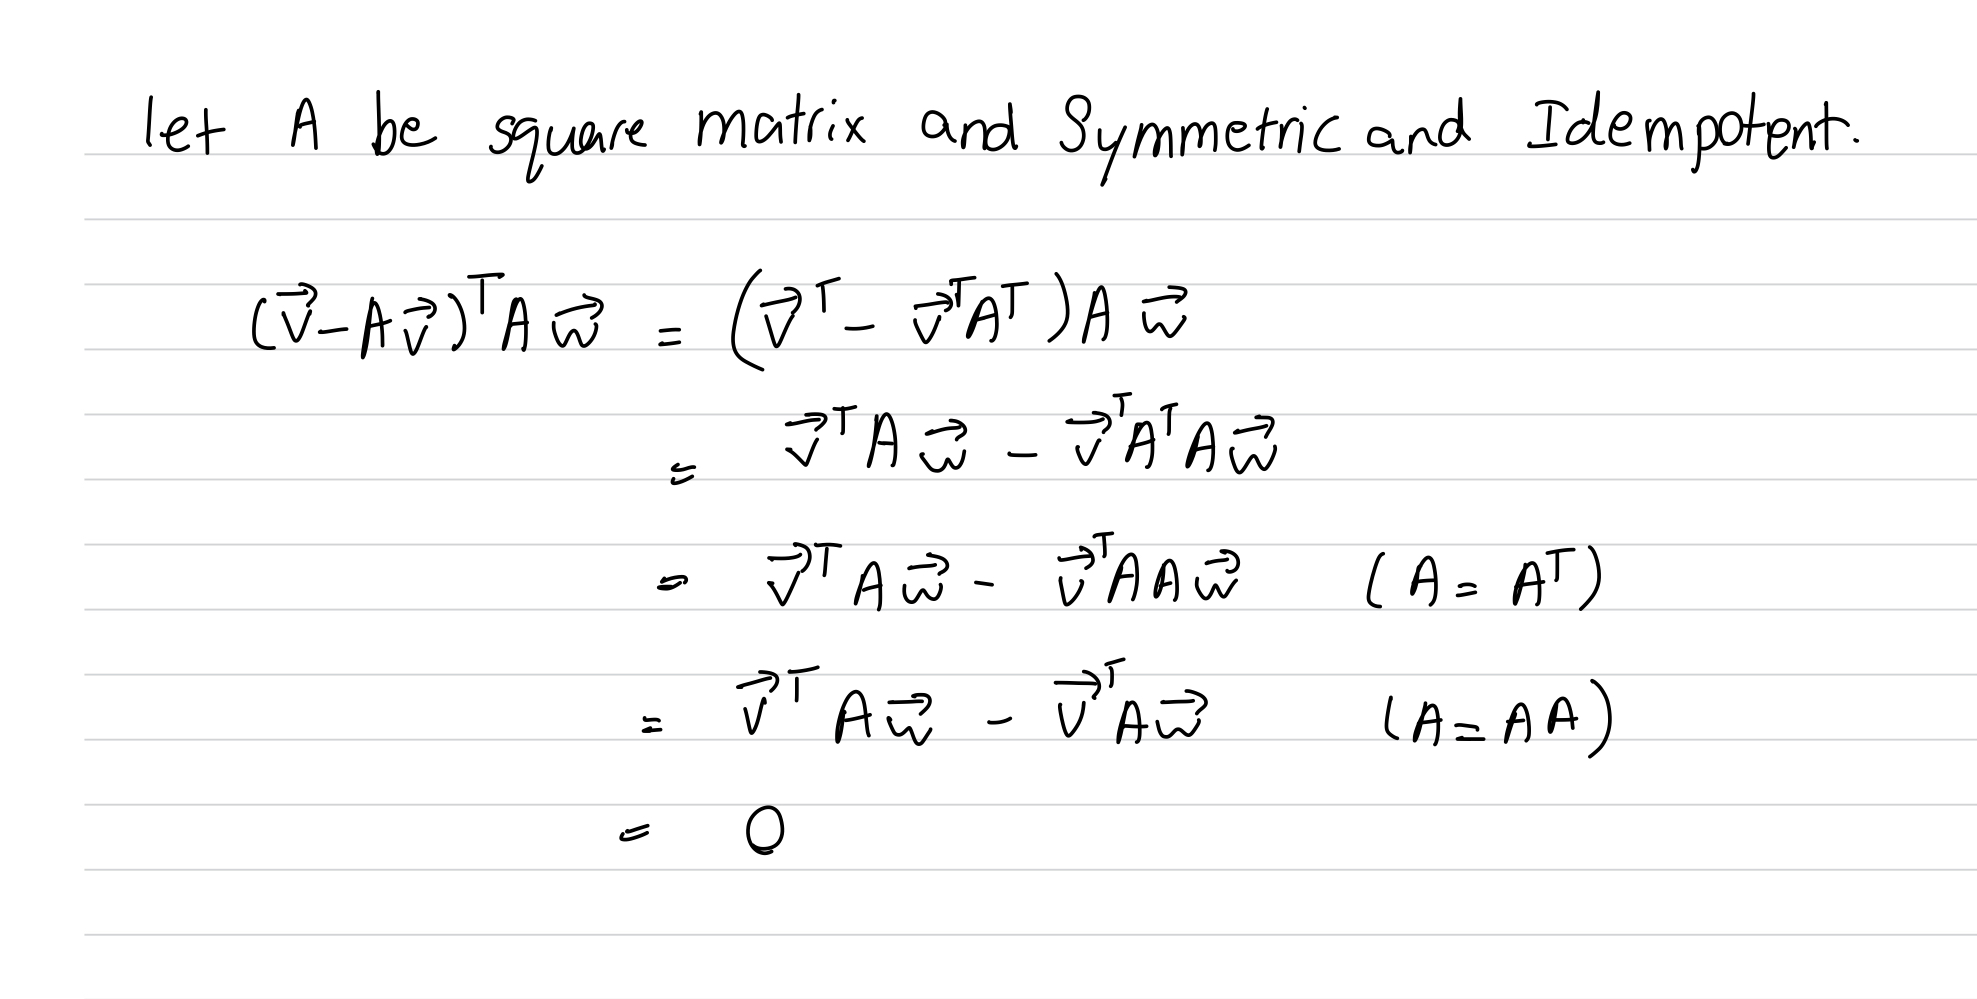
\includegraphics[width=0.75\linewidth]{JPEG image-46C2-ACDB-30-0.jpeg}
    \caption{Problem 2 f}
    \label{fig:enter-label}
\end{figure}

\hardsubproblem{[MA] Prove the converse of the previous question: that if a square matrix is an orthogonal projection matrix, then it must be both symmetric and idempotent.}\spc{4}

\easysubproblem{Prove that $I_n$ is an orthogonal projection matrix $\forall n$.}\spc{3}

\( I_n \) is symmetric, since 
\[
I_n^T = I_n
\]
as it only has a diagonal matrix of 1s.

\( I_n \) is idempotent, since
\[
I_n^2 = I_n.
\]

Thus, \( I_n \) is an orthogonal projection matrix.

We can also prove this in another way:

\[
(\vec{v} - P\vec{v})^T (P\vec{w}) = 0
\]

\[
(\vec{v} - I_n \vec{v})^T (I_n \vec{w}) = 0
\]

\[
(\vec{v} - \vec{v})^T (\vec{w}) = 0
\]

\[
(\mathbf{0})^T (\vec{w}) = 0
\]

\[
0 = 0
\]

Thus, \( I_n \) is an orthogonal projection matrix.


\easysubproblem{What subspace does $I_n$ project onto?}\spc{3}

$I_n$ projects onto $R_n$ space.



\easysubproblem{Consider least squares linear regression using a design matrix $X$ with rank $p + 1$. What are the degrees of freedom in the resulting model? What does this mean?}\spc{3}

The degrees of freedom is p+1 and it means the number of linearly independent columns.


%\easysubproblem{If you are orthogonally projecting the vector $\y$ onto the column space of $X$ which is of rank $p + 1$, derive the formula for $\proj{\colsp{X}}{\y}$. Is this the same as in OLS?}\spc{8}

\hardsubproblem{We saw that the perceptron is an \textit{iterative algorithm}. This means that it goes through multiple iterations in order to converge to a closer and closer $\bv{w}$. Why not do the same with linear least squares regression? Consider the following. Regress $\y$ using $\X$ to get $\yhat$. This generates residuals $\e$ (the leftover piece of $\y$ that wasn't explained by the regression's fit, $\yhat$). Now try again! Regress $\e$ using $\X$ and then get new residuals $\e_{new}$. Would $\e_{new}$ be closer to $\bv{0}_n$ than the first $\e$? That is, wouldn't this yield a better model on iteration \#2? Yes/no and explain.}\spc{8}




\intermediatesubproblem{Prove that $\Q^\top = \Q^{-1}$ where $\Q$ is an orthonormal matrix such that $\colsp{\Q} = \colsp{\X}$ and $\Q$ and $\X$ are both matrices $\in \reals^{n \times (p+1)}$ and $n = p+1$ in this case to ensure the inverse is defined. Hint: this is purely a linear algebra exercise and it's a one-liner.}\spc{2}

\[
Q^T Q = I, \quad \text{since } Q \text{ is a square matrix and it is also full rank, there is a } Q^{-1}
\]

\[
Q^T = Q^{-1}
\]


\easysubproblem{Prove that the least squares projection $\H = \XXtXinvXt = \Q\Q^\top$. Justify each step.}\spc{4}

\begin{figure}[H]
    \centering
    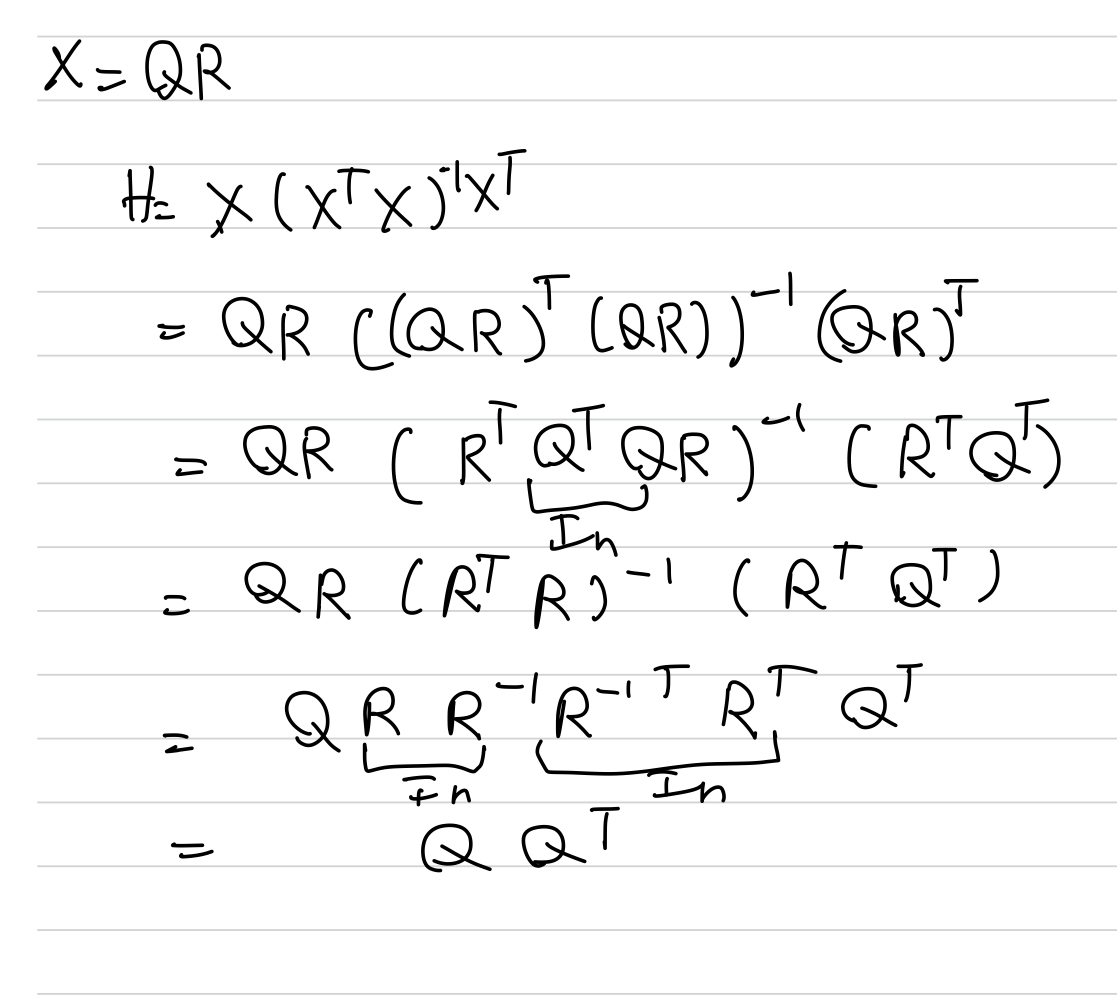
\includegraphics[width=0.7\linewidth]{IMG_C1C12252007B-1.jpeg}
    \caption{Enter Caption}
    \label{fig:enter-label}
\end{figure}


\hardsubproblem{[MA] This problem is independent of the others. Let $H$ be an orthogonal projection matrix. Prove that $\rank{\H} =\tr{\H}$. Hint: you will need to use facts about eigenvalues and the eigendecomposition of projection matrices.}\spc{8}

\intermediatesubproblem{Prove that an orthogonal projection onto the $\colsp{\Q}$ is the same as the sum of the projections onto each column of $\Q$.}\spc{7}

\begin{figure}[H]
    \centering
    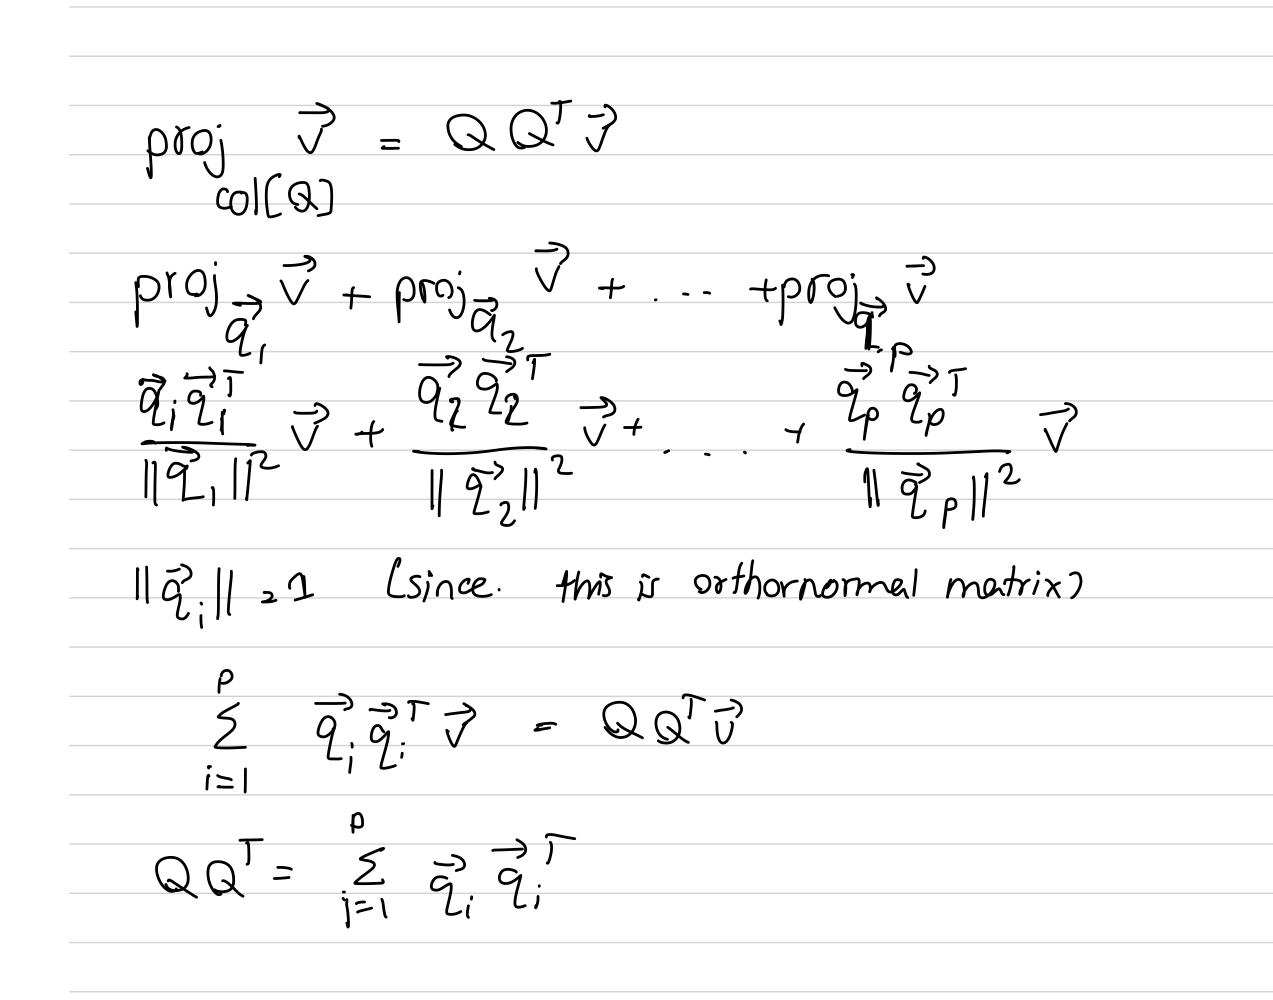
\includegraphics[width=0.75\linewidth]{IMG_F5C4FFE89889-1.jpeg}
    \caption{Enter Caption}
    \label{fig:enter-label}
\end{figure}

\easysubproblem{Explain why adding a new column to $\X$ results in no change to SST.}\spc{2}

Because SST is the summation of the square of $y_i$ - $\bar{y}$ and if we add more column to $\X$, $y_i$ or $\bar{y}$ doesn't change and only $\hat{y}$ change.

\intermediatesubproblem{Prove that adding a new column to $\X$ results in SSR increasing.}\spc{4}

\begin{figure}[H]
    \centering
    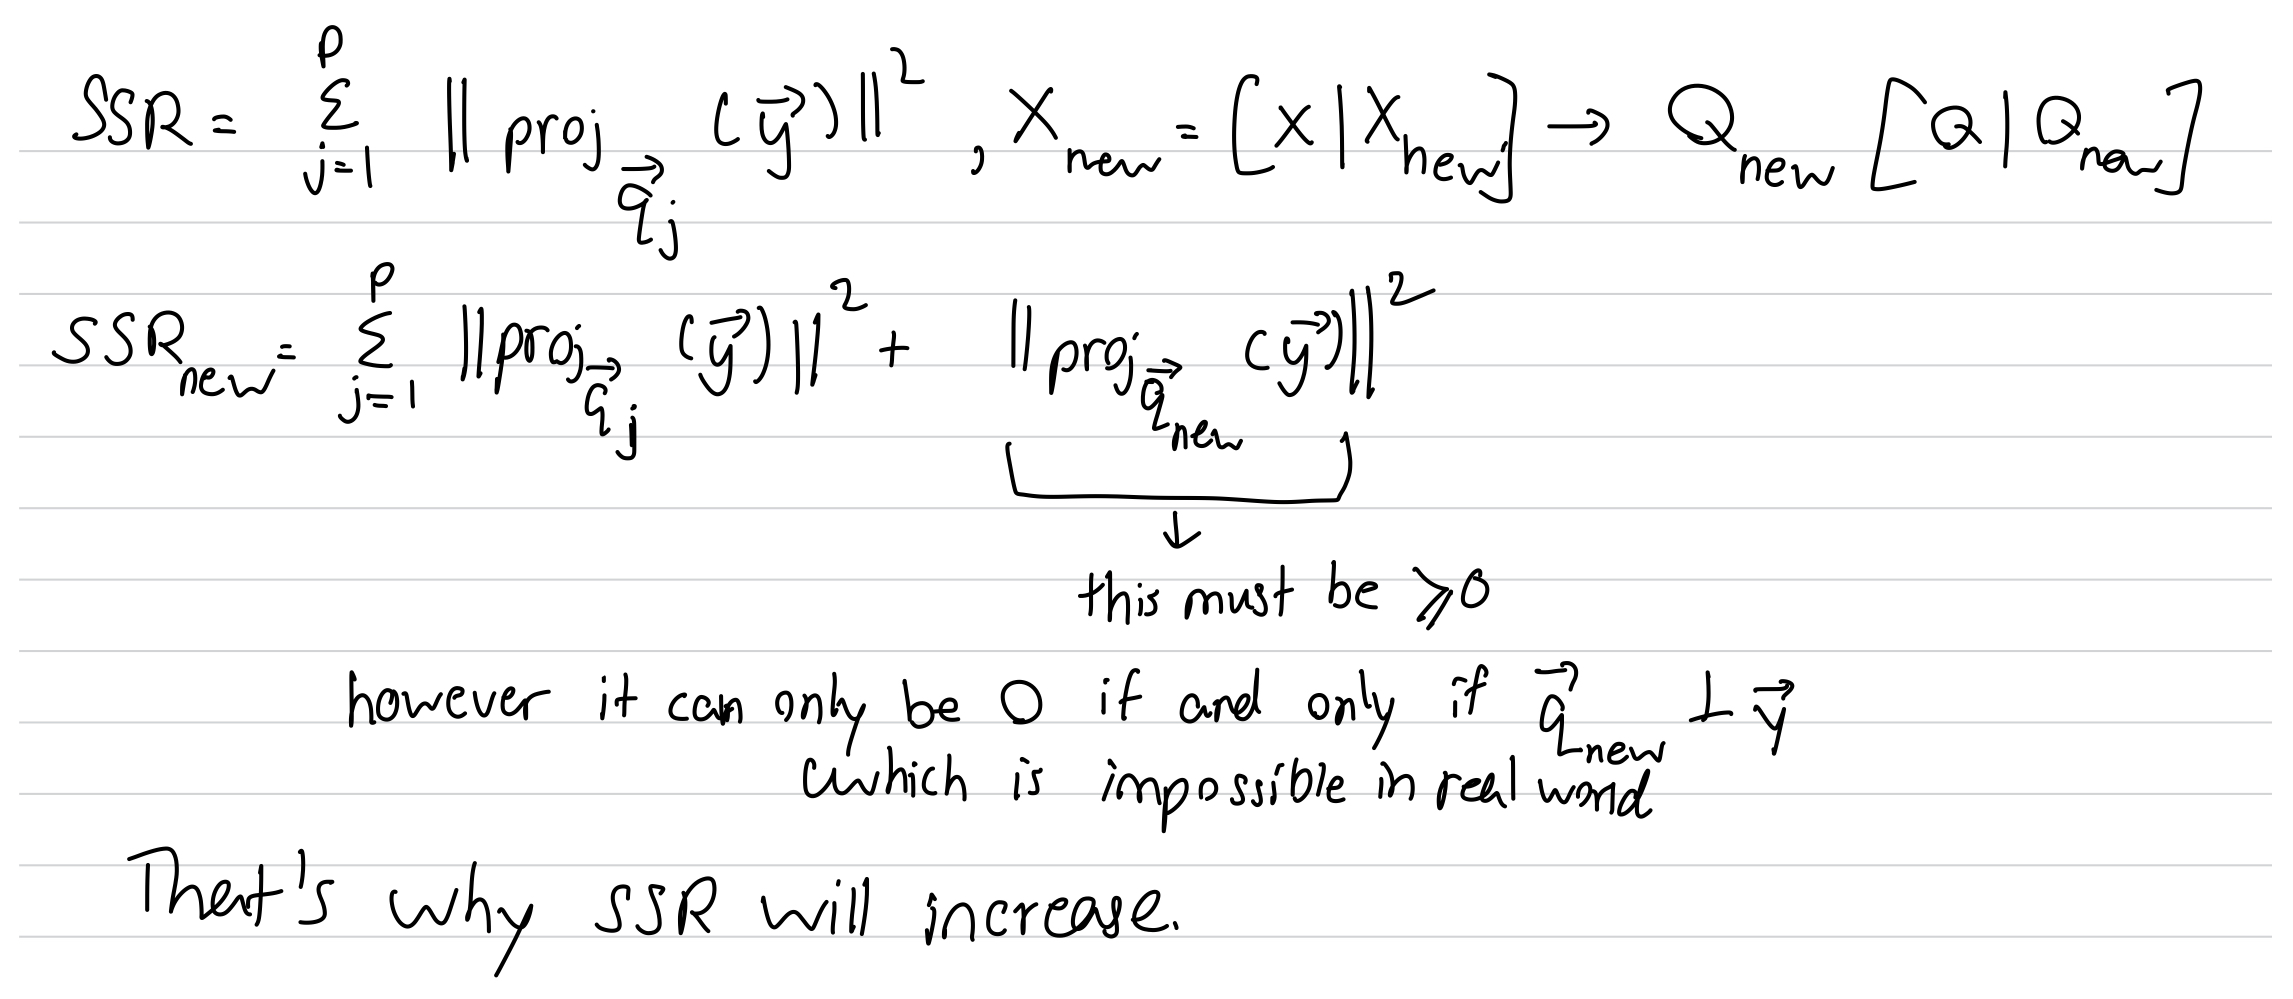
\includegraphics[width=0.75\linewidth]{IMG_8D864DBE0B68-1.jpeg}
    \caption{Enter Caption}
    \label{fig:enter-label}
\end{figure}

\intermediatesubproblem{What is overfitting? Use what you learned in this problem to frame your answer.}\spc{2}

Overfitting is that when you add junk features which doesn't contribute to your approximation of z's to your data set to train and after you train, you may see that the SSR increases, SSE decreases and $R^2$ increases. When you see that you might think that the model is better. However, it is worse when you check with out of sample data set.



\easysubproblem{Why are the \qu{in-sample} error metrics $R^2$ and SSE dishonest? Note: I'm leaving out MSE and RMSE as they attempt to be honest by increasing as $p$ increases due to the denominator.}\spc{3}

Because SSE and $R^2$ will increase because when you add a new column the SSR will always increase (from the justification from problem 2(q)) and so it will not tell that your model is good or bad.

\easysubproblem{How can we provide honest error metrics for $R^2$, SSE? It may help to draw a picture of the procedure.}\spc{14}

We can provide honest error metrics for $R^2$ by splitting the data into two part, training dataset and testing data set. So, you can use testing data set to get out of simple prediction and you will get an oos error from that. That oose can validate your model if it overfit or not.


\easysubproblem{The procedure in the previous question produces highly variable honest error metrics. Can you change the procedure slightly to reduce the variation in the honest error metrics? What is this procedure called and how is it done?}\spc{6}

Yes. I can change the procedure slightly to reduce the variation in the honest error metrics. This procedure is called "Cross Validation" or "K-fold CV". The procedure is following: first split 20\% of your data to testing data and the rest are training data. Then, you find the error of first 20\% of the data. Then, put that data into the data set and split another different 20\% of the data for the testing data and repeat the process. In the end, you will get a vector of errors which is length n and you can compute oos metrics using them.



\end{enumerate}


\problem{These are some questions related to validation.}

\begin{enumerate}

\easysubproblem{Assume you are doing one train-test split where you build the model on the training set and validate on the test set. What does the constant $K$ control? And what is its tradeoff?}\spc{4}

K control the proportion of the number of original data set and the number of testing data set. The trade off is that the smaller the proportion in training data set, there will be more estimation error as we don't get enough n. this mean that your oos error metric is too high. The higher the prop of training data. your oos metrics are highly variable, thereby hard to trust.

\easysubproblem{What problem does $K$-fold CV try to solve?}\spc{5}

They are trying to solve the problem of unstable and highly variate oos metrics if K is large.

\hardsubproblem{[MA] Theoretically, how does $K$-fold CV solve this problem? The Internet is your friend.}\spc{5}

%\intermediatesubproblem{Assume you are doing one train-test split where you build the model on the training set and validate on the test set. If $n$ was very large so that there would be trivial misspecification error even when using $K=2$, would there be any benefit at all to increasing $K$ if your objective was to estimate generalization error? Explain.}\spc{4}

\end{enumerate}

\end{document}



